%\documentclass[11pt]{beamer}
\documentclass[11pt,handout,aspectratio=1610]{beamer}

\usepackage[utf8]{inputenc}
\usepackage[T1]{fontenc}
\usepackage[spanish]{babel}
\usepackage{latexsym} 
\usepackage{amsmath}
\usepackage{amsfonts}
\usepackage{amssymb}
\usepackage{esint}
\usepackage{array}
\usepackage{multirow}
\usepackage{xcolor}
\usepackage{graphicx}
\usepackage{tikz}
\usepackage{tikz-3dplot}
\usetikzlibrary{babel}
\usetikzlibrary{calc,patterns,decorations.pathmorphing,decorations.markings}
\usepackage{xcolor}
\usepackage{epstopdf}
\usepackage[nointegrals]{wasysym}
\usepackage{hyperref}
\usepackage{cancel}

\usetheme{Berkeley}
\usecolortheme{seahorse}
\uselanguage{Spanish}

\newcommand{\sgn}{\mathop{\text{sgn}}}
\newcommand{\diff}[0]{\text{d}}
\newcommand{\fdiff}[2]{\dfrac{\text{d} #1}{\text{d} #2}}
\newcommand{\pdiff}[2]{\frac{\partial #1}{\partial #2}}
\newcommand{\fddiff}[2]{\frac{\text{d^2} #1}{\text{d} #2^2}}
\newcommand{\degr}[0]{^{\circ}}
\newcommand{\chel}[4]{^{#1}_{#2}\text{#3}^{#4}}
\newcommand{\valmed}[1]{\left\langle #1 \right\rangle}
\newcommand{\E}[1]{\times 10^{#1}}
%\renewcommand{\vec}[1]{\text{\textbf{#1}}}
\newcommand{\ver}[1]{\hat{\vec{#1}}}
\newcommand{\vecg}[1]{\boldsymbol{#1}}
\newcommand{\iu}{\text{i}}
\newcommand{\norm}[1]{\left\vert\left\vert #1 \right\vert\right\vert}
\newcommand{\abs}[1]{\left\vert #1 \right\vert}
\newcommand{\tens}[1]{\mathbb{#1}}
\newcommand{\rr}{\mathbb{R}}
\newcommand{\logoUNAHUR}{
\includegraphics[scale=0.15]{/home/shluna/Proyectos/Clases_Fisica_III/imgs/logo-universidad-nacional-de-hurlingham_preview_rev_1.png}}
\newcommand{\vs}{\vspace{11pt}}
\newcommand{\un}[1]{\text{#1}}
\renewcommand{\arraystretch}{1.2}

\title{Sistemas de partículas y cuerpo rígido}
\subtitle{Unidad 2}
\author{Física III}
\institute{Instituto de Tecnología e Ingeniería \\ \vspace{0.25cm} Universidad Nacional de Hurlingham}
\date{Tercera parte}
\logo{\logoUNAHUR}

\AtBeginSection[]{
  \begin{frame}
  \vfill
  \centering
  \begin{beamercolorbox}[sep=8pt,center,shadow=true,rounded=true]{title}
    \usebeamerfont{title}\insertsectionhead\par%
  \end{beamercolorbox}
  \vfill
  \end{frame}
}

\tdplotsetmaincoords{70}{110}

\begin{document}

\renewcommand{\tablename}{Tabla}

\frame{\titlepage}

\begin{frame}{En esta clase veremos:}
    \tableofcontents
\end{frame}

\section{Ecuación de movimiento del CR}

\begin{frame}{Ecuación de movimiento rotacional de un cuerpo rígido}

    En general, cada partícula que forma un cuerpo rígido puede estar sometido a fuerzas externas e internas.

    \vs

    Consideremos la \emph{fuerza resultante} sobre una partícula arbitraria del cuerpo rígido.

    \vs

    \begin{columns}
        \begin{column}{0.5\textwidth}
            \begin{figure}
                \centering
                \begin{tikzpicture}    
                    \pgfmathsetseed{3}
                    \draw[fill=gray!40] plot [smooth cycle, samples=8,domain={1:8}](\x*360/8+5*rnd:0.8cm+1.5cm*rnd) node at (0,0) {};
                    \draw[dashed] (0,0) circle (1.2);
                    \begin{scope}[rotate=45]
                    \draw[thick,-latex] (0,0) -- node[anchor=north]{\scriptsize $\vec{r}_i$} (0:1.2);
                    \fill[black] (0,0) circle (0.3mm) node[anchor=north]{\scriptsize $O$};
                    \fill[black] (0:1.2) circle (0.3mm) node[anchor=west]{\scriptsize $m_i$};
                    \draw[thick,-latex,blue] (0:1.2) -- (0.5,0.8) node[anchor=north east]{\scriptsize $\vec{F}^{(i)}$};
                    \draw[thick,-latex,blue] (0:1.2) -- node[anchor=south west]{\scriptsize $\vec{F}_\text{t}^{(i)}$} (1.2,0.8);
                    \draw[thick,-latex,blue] (0:1.2) -- node[anchor=north west]{\scriptsize $\vec{F}_\text{c}^{(i)}$} (0.5,0);
                    \draw[dashed,blue] (0.5,0) -- (0.5,0.8) -- (1.2,0.8);
                    \end{scope}
                \end{tikzpicture}
            \end{figure}
        \end{column}
        \begin{column}{0.5\textwidth}
            La fuerza resultante $\vec{F}^{(i)}$ que actúa sobre la partícula $i$, de masa $m_i$ se puede descomponer en sus componentes tangencial, $\vec{F}_\text{t}^{(i)}$, y centrípeta, $\vec{F}_\text{c}^{(i)}$.

            \vs 

            De las dos componentes, solamente la tangencial es la que produce un efecto de rotación, es decir, un torque o un momento.
        \end{column}
    \end{columns}

\end{frame}

\begin{frame}{Ecuación de movimiento rotacional de un cuerpo rígido}

    El torque o momento producido por la fuerza $\vec{F}^{(i)}$ que actúa sobre la partícula $i$, respecto del punto $O$, es: $$\vec{T}^{(i)} = \vec{r}_i \times \vec{F}^{(i)} = \vec{r}_i \times \vec{F}_\text{t}^{(i)}.$$

    \begin{columns}
        \begin{column}{0.5\textwidth}
            \begin{figure}
                \centering
                \begin{tikzpicture}    
                    \pgfmathsetseed{3}
                    \draw[fill=gray!40] plot [smooth cycle, samples=8,domain={1:8}](\x*360/8+5*rnd:0.8cm+1.5cm*rnd) node at (0,0) {};
                    \draw[dashed] (0,0) circle (1.2);
                    \begin{scope}[rotate=45]
                    \draw[thick,-latex] (0,0) -- node[anchor=north]{\scriptsize $\vec{r}_i$} (0:1.2);
                    \fill[black] (0,0) circle (0.3mm) node[anchor=north]{\scriptsize $O$};
                    \fill[black] (0:1.2) circle (0.3mm) node[anchor=west]{\scriptsize $m_i$};
                    \draw[thick,-latex,blue] (0:1.2) -- (0.5,0.8) node[anchor=north east]{\scriptsize $\vec{F}^{(i)}$};
                    \draw[thick,-latex,blue] (0:1.2) -- node[anchor=south west]{\scriptsize $\vec{F}_\text{t}^{(i)}$} (1.2,0.8);
                    \draw[thick,-latex,blue] (0:1.2) -- node[anchor=north west]{\scriptsize $\vec{F}_\text{c}^{(i)}$} (0.5,0);
                    \draw[dashed,blue] (0.5,0) -- (0.5,0.8) -- (1.2,0.8);
                    \end{scope}
                \end{tikzpicture}
            \end{figure}
        \end{column}
        \begin{column}{0.5\textwidth}
            Habíamos visto que este torque produce una aceleración angular $\alpha_i$ sobre la partícula, esto es: $$T_i = I_i \, \alpha_i$$ donde $T_i$ y $\alpha_i$ son las componentes $z$ del torque y de la aceleración angular, respectivamente, e $I_i = m_i \, r_i^2$ es el momento de inercia de la partícula.
        \end{column}
    \end{columns}

\end{frame}

% \begin{frame}{Ecuación de movimiento rotacional de un cuerpo rígido}

%     \begin{columns}
%         \begin{column}{0.5\textwidth}
%             \begin{figure}
%                 \centering
%                 \begin{tikzpicture}    
%                     \pgfmathsetseed{3}
%                     \draw[fill=gray!40] plot [smooth cycle, samples=8,domain={1:8}](\x*360/8+5*rnd:0.8cm+1.5cm*rnd) node at (0,0) {};
%                     \draw[dashed] (0,0) circle (1.2);
%                     \begin{scope}[rotate=45]
%                     \draw[thick,-latex] (0,0) -- node[anchor=north]{\scriptsize $\vec{r}_i$} (0:1.2);
%                     \fill[black] (0,0) circle (0.3mm) node[anchor=north]{\scriptsize $O$};
%                     \fill[black] (0:1.2) circle (0.3mm) node[anchor=west]{\scriptsize $i$};
%                     \draw[thick,-latex,blue] (0:1.2) -- (0.5,0.8) node[anchor=north east]{\scriptsize $\vec{F}^{(i)}$};
%                     \draw[thick,-latex,blue] (0:1.2) -- node[anchor=south west]{\scriptsize $\vec{F}_\text{t}^{(i)}$} (1.2,0.8);
%                     \draw[thick,-latex,blue] (0:1.2) -- node[anchor=north west]{\scriptsize $\vec{F}_\text{c}^{(i)}$} (0.5,0);
%                     \draw[dashed,blue] (0.5,0) -- (0.5,0.8) -- (1.2,0.8);
%                     \end{scope}
%                 \end{tikzpicture}
%             \end{figure}
%         \end{column}
%         \begin{column}{0.5\textwidth}
%             En virtud de la segunda ley de Newton: $$F_\text{t}^{(i)} = m_i \, a_\text{t}^{(i)}$$ Además, $$a_\text{t}^{(i)} = r_i \, \alpha_i$$ donde $\alpha_i$ es la aceleración angular de la partícula $i$.
%         \end{column}
%     \end{columns}

% \end{frame}

% \begin{frame}{Ecuación de movimiento rotacional de un cuerpo rígido}

%     \begin{columns}
%         \begin{column}{0.5\textwidth}
%             \begin{figure}
%                 \centering
%                 \begin{tikzpicture}    
%                     \pgfmathsetseed{3}
%                     \draw[fill=gray!40] plot [smooth cycle, samples=8,domain={1:8}](\x*360/8+5*rnd:0.8cm+1.5cm*rnd) node at (0,0) {};
%                     \draw[dashed] (0,0) circle (1.2);
%                     \begin{scope}[rotate=45]
%                     \draw[thick,-latex] (0,0) -- node[anchor=north]{\scriptsize $\vec{r}_i$} (0:1.2);
%                     \fill[black] (0,0) circle (0.3mm) node[anchor=north]{\scriptsize $O$};
%                     \fill[black] (0:1.2) circle (0.3mm) node[anchor=west]{\scriptsize $i$};
%                     \draw[thick,-latex,blue] (0:1.2) -- (0.5,0.8) node[anchor=north east]{\scriptsize $\vec{F}^{(i)}$};
%                     \draw[thick,-latex,blue] (0:1.2) -- node[anchor=south west]{\scriptsize $\vec{F}_\text{t}^{(i)}$} (1.2,0.8);
%                     \draw[thick,-latex,blue] (0:1.2) -- node[anchor=north west]{\scriptsize $\vec{F}_\text{c}^{(i)}$} (0.5,0);
%                     \draw[dashed,blue] (0.5,0) -- (0.5,0.8) -- (1.2,0.8);
%                     \end{scope}
%                 \end{tikzpicture}
%             \end{figure}
%         \end{column}
%         \begin{column}{0.5\textwidth}
%          En consecuencia, $$F_\text{t}^{(i)} = m_i \, r_i \, \alpha_i$$ y, por lo tanto: $$T^{(i)} = m_i \, r_i^2 \, \alpha_i$$
%         \end{column}
%     \end{columns}

% \end{frame}

% \begin{frame}{Ecuación de movimiento rotacional de un cuerpo rígido}

%     \begin{columns}
%         \begin{column}{0.5\textwidth}
%             \begin{figure}
%                 \centering
%                 \begin{tikzpicture}    
%                     \pgfmathsetseed{3}
%                     \draw[fill=gray!40] plot [smooth cycle, samples=8,domain={1:8}](\x*360/8+5*rnd:0.8cm+1.5cm*rnd) node at (0,0) {};
%                     \draw[dashed] (0,0) circle (1.2);
%                     \begin{scope}[rotate=45]
%                     \draw[thick,-latex] (0,0) -- node[anchor=north]{\scriptsize $\vec{r}_i$} (0:1.2);
%                     \fill[black] (0,0) circle (0.3mm) node[anchor=north]{\scriptsize $O$};
%                     \fill[black] (0:1.2) circle (0.3mm) node[anchor=west]{\scriptsize $i$};
%                     \draw[thick,-latex,blue] (0:1.2) -- (0.5,0.8) node[anchor=north east]{\scriptsize $\vec{F}^{(i)}$};
%                     \draw[thick,-latex,blue] (0:1.2) -- node[anchor=south west]{\scriptsize $\vec{F}_\text{t}^{(i)}$} (1.2,0.8);
%                     \draw[thick,-latex,blue] (0:1.2) -- node[anchor=north west]{\scriptsize $\vec{F}_\text{c}^{(i)}$} (0.5,0);
%                     \draw[dashed,blue] (0.5,0) -- (0.5,0.8) -- (1.2,0.8);
%                     \end{scope}
%                 \end{tikzpicture}
%             \end{figure}
%         \end{column}
%         \begin{column}{0.5\textwidth}
%             Podemos entonces calcular el momento resultante sobre el cuerpo rígido como la suma de los momentos aplicados a cada partícula: $$T = \sum_{i=1}^N T^{(i)} = \sum_{i=1}^N m_i \, r_i^2 \, \alpha_i$$ 
%         \end{column}
%     \end{columns}

% \end{frame}

% \begin{frame}{Ecuación de movimiento rotacional de un cuerpo rígido}

%     \begin{columns}
%         \begin{column}{0.5\textwidth}
%             \begin{figure}
%                 \centering
%                 \begin{tikzpicture}    
%                     \pgfmathsetseed{3}
%                     \draw[fill=gray!40] plot [smooth cycle, samples=8,domain={1:8}](\x*360/8+5*rnd:0.8cm+1.5cm*rnd) node at (0,0) {};
%                     \draw[dashed] (0,0) circle (1.2);
%                     \begin{scope}[rotate=45]
%                     \draw[thick,-latex] (0,0) -- node[anchor=north]{\scriptsize $\vec{r}_i$} (0:1.2);
%                     \fill[black] (0,0) circle (0.3mm) node[anchor=north]{\scriptsize $O$};
%                     \fill[black] (0:1.2) circle (0.3mm) node[anchor=west]{\scriptsize $i$};
%                     \draw[thick,-latex,blue] (0:1.2) -- (0.5,0.8) node[anchor=north east]{\scriptsize $\vec{F}^{(i)}$};
%                     \draw[thick,-latex,blue] (0:1.2) -- node[anchor=south west]{\scriptsize $\vec{F}_\text{t}^{(i)}$} (1.2,0.8);
%                     \draw[thick,-latex,blue] (0:1.2) -- node[anchor=north west]{\scriptsize $\vec{F}_\text{c}^{(i)}$} (0.5,0);
%                     \draw[dashed,blue] (0.5,0) -- (0.5,0.8) -- (1.2,0.8);
%                     \end{scope}
%                 \end{tikzpicture}
%             \end{figure}
%         \end{column}
%         \begin{column}{0.5\textwidth}
%             Pero, como la aceleración angular es la misma para todas las partículas ($\alpha_i = \alpha$), esta puede sacarse como factor común: $$T = \left(\sum_{i=1}^N m_i \, r_i^2\right) \alpha$$
%         \end{column}
%     \end{columns}

% \end{frame}

% \begin{frame}{Ecuación de movimiento rotacional de un cuerpo rígido}

%     \begin{columns}
%         \begin{column}{0.5\textwidth}
%             \begin{figure}
%                 \centering
%                 \begin{tikzpicture}    
%                     \pgfmathsetseed{3}
%                     \draw[fill=gray!40] plot [smooth cycle, samples=8,domain={1:8}](\x*360/8+5*rnd:0.8cm+1.5cm*rnd) node at (0,0) {};
%                     \draw[dashed] (0,0) circle (1.2);
%                     \begin{scope}[rotate=45]
%                     \draw[thick,-latex] (0,0) -- node[anchor=north]{\scriptsize $\vec{r}_i$} (0:1.2);
%                     \fill[black] (0,0) circle (0.3mm) node[anchor=north]{\scriptsize $O$};
%                     \fill[black] (0:1.2) circle (0.3mm) node[anchor=west]{\scriptsize $i$};
%                     \draw[thick,-latex,blue] (0:1.2) -- (0.5,0.8) node[anchor=north east]{\scriptsize $\vec{F}^{(i)}$};
%                     \draw[thick,-latex,blue] (0:1.2) -- node[anchor=south west]{\scriptsize $\vec{F}_\text{t}^{(i)}$} (1.2,0.8);
%                     \draw[thick,-latex,blue] (0:1.2) -- node[anchor=north west]{\scriptsize $\vec{F}_\text{c}^{(i)}$} (0.5,0);
%                     \draw[dashed,blue] (0.5,0) -- (0.5,0.8) -- (1.2,0.8);
%                     \end{scope}
%                 \end{tikzpicture}
%             \end{figure}
%         \end{column}
%         \begin{column}{0.5\textwidth}
%             $$T = \left(\sum_{i=1}^N m_i \, r_i^2\right) \alpha$$ La cantidad entre paréntesis se conoce como \emph{momento de inercia del sistema de partículas} y se lo denota $I$, esto es: $$I = \sum_{i=1}^N m_i \, r_i^2$$
%         \end{column}
%     \end{columns}

% \end{frame}

\begin{frame}{Ecuación de movimiento rotacional de un cuerpo rígido}

    Por otro lado, tenemos que el momento angular del cuerpo rígido es $$\vec{L} = I \, \vec{\omega}$$ Podemos entonces preguntarnos qué es lo que causa la variación o cambio en el tiempo de este vector. Para responder esta pregunta podemos comenzar derivando la expresión de $\vec{L}$ con respecto al tiempo: $$ \fdiff{\vec{L}}{t} = I \fdiff{\vec{\omega}}{t}$$ El momento de inercia del cuerpo rígido es constante puesto que la masa de cada partícula es constante, así como también lo son las distancias entre ellas, en general (por definición del cuerpo rígido), y en particular la distancia de cada una al eje alrededor del cual gira el cuerpo rígido.

\end{frame}

\begin{frame}{Ecuación de movimiento rotacional de un cuerpo rígido}

    Independientemente de la causa, la derivada temporal de la velocidad angular es lo que conocemos como \emph{aceleración angular} ($\vec{\alpha}$): $$ \vec{\alpha} = \fdiff{\vec{\omega}}{t}$$ la cual, como cabe suponer, es la aceleración angular de todo el cuerpo rígido. Entonces, tenemos que: $$ \fdiff{\vec{L}}{t} = I \vec{\alpha} $$ 
 
\end{frame}

\begin{frame}{Ecuación de movimiento rotacional de un cuerpo rígido}   
    
    Si ahora tenemos en cuenta la expresión del momento de inercia del cuerpo rígido: $$ I = \sum_{i=1}^{N} I_i $$ la derivada temporal del momento angular del cuerpo rígido se puede expresar también como: $$ \fdiff{\vec{L}}{t} = \left(\sum_{i=1}^{N} I_i \right) \vec{\alpha} $$ A continuación, podemos distribuir la aceleración angular dentro de la suma entre paréntesis: $$ \fdiff{\vec{L}}{t} = \sum_{i=1}^{N} \left(I_i\vec{\alpha}\right) $$

\end{frame}

\begin{frame}{Ecuación de movimiento rotacional de un cuerpo rígido}

    Ahora bien, en virtud de su definición, la aceleración angular del cuerpo rígido debe ser la misma para cada partícula que lo compone, esto es: $$ \vec{\alpha} = \vec{\alpha}_1 = \vec{\alpha}_2 = \ldots = \vec{\alpha}_i = \ldots = \vec{\alpha}_N $$ En consecuencia, podemos escribir: $$ \fdiff{\vec{L}}{t} = \sum_{i=1}^{N} \left(I_i \vec{\alpha}_i \right), $$ de donde se ve claramente que la magnitud entre paréntesis no es otra cosa que el torque aplicado sobre la partícula $i$: $$\vec{T}_i = I_i \, \vec{\alpha}_i$$

\end{frame}

\begin{frame}{Ecuación de movimiento rotacional de un cuerpo rígido}

    Entonces, vemos que, por un lado: $$ \fdiff{\vec{L}}{t} = \vec{T}$$ donde ahora $$ \vec{T} = \sum_{i=1}^{N} \vec{T}_i $$ es el \emph{torque resultante} aplicado sobre todo el cuerpo rígido, es decir, la suma vectorial de los torque aplicados a cada partícula. Por otro lado, teníamos que $$ \fdiff{\vec{L}}{t} = I \vec{\alpha} $$
    
\end{frame}

\begin{frame}{Ecuación de movimiento rotacional de un cuerpo rígido}

    Finalmente, igualando las dos expresiones de la derivada temporal del momento angular, llegamos a la 
    \begin{block}{Ecuación de movimiento rotacional del cuerpo rígido}
        $$\vec{T} = I \, \vec{\alpha}$$ donde $\vec{T}$ es el torque resultante, $I$ es el momento de inercia del cuerpo rígido y $\vec{\alpha}$ es su aceleración angular.
    \end{block} Esta es la ecuación que describe la dinámica rotacional de un cuerpo rígido. En otras palabras, es la versión de la segunda ley de Newton para el movimiento de rotación. $$\vec{F} = m \, \vec{a}$$ donde $\vec{T}$ juega el papel de la fuerza, $I$ el de la masa y $\vec{\alpha}$ el de la aceleración lineal.

\end{frame}

\begin{frame}{Ecuación de movimiento rotacional de un cuerpo rígido}

\begin{block}{Concepto de momento de inercia}
    En virtud de la ecuación de movimiento rotacional, $\vec{T} = I \, \vec{\alpha}$, el momento de inercia ($I$) mide la resistencia que ofrece un cuerpo a adquirir una aceleración angular $\vec{\alpha}$ cuando se le aplica un torque o momento $\vec{T}$.
\end{block}

\end{frame}

\section{Conservación del momento angular}

\begin{frame}{Momento angular de un cuerpo rígido}

    Una consecuencia inmediata de la ecuación $$ \frac{\text{d}\vec{L}}{\text{d}t} = \vec{T}$$ es que si el torque o momento resultante de las fuerzas aplicadas a un cuerpo rígido es nulo, entonces: $$ \frac{\text{d}\vec{L}}{\text{d}t} = \vec{0}$$ Lo cual implica que el momento angular se conserva en el tiempo. 

    \vs 

    Esto puede corresponder a que no hay fuerza alguna que pueda producir un torque, o bien que la sumatoria de los torques producidos por algunas o todas las fuerzas aplicadas al cuerpo es igual a cero.

\end{frame}

\begin{frame}{Momento angular de un cuerpo rígido}

    Así, llegamos al:
    \begin{block}{Teorema de conservación del momento angular}
        Si el momento resultante de las fuerzas \emph{externas} aplicadas a un sistema de partículas es nulo, entonces se conserva el momento angular total del sistema.
    \end{block}

\end{frame}

\section{Torque resultante y torque de la resultante}

\begin{frame}{Torque resultante y torque de la resultante}

    Cuando trabajábamos con un conjunto de fuerzas aplicadas a una masa puntual, determinábamos la fuerza resultante como la suma vectorial de las fuerzas aplicadas y considerábamos que esta estaba aplicada sobre la masa puntual. Así, la resultante produce el mismo efecto dinámico que e conjunto de fuerzas aplicadas. 
    
    \vs
    
    Ahora, para el estudio del movimiento de rotación de un cuerpo extenso, no solamente debemos considerar las fuerzas en sí sino que también hay que tener en cuenta dónde está aplicada cada una de ellas.

    \vs 

    El objetivo es determinar las coordenadas $\left(x_R; y_R\right)$ del punto donde debe aplicarse la resultante para producir un torque igual al torque resultante.
    
\end{frame}

\begin{frame}{Torque resultante y torque de la resultante}

    Consideremos un sistema sencillo formado por dos fuerzas, $\vec{F}_1$ y $\vec{F}_2$, aplicadas a un cuerpo rígido en los puntos ubicados por los vectores de posición $\vec{r}_1$ y $\vec{r}_2$, respectivamente. Las componentes cartesianas de estos vectores son:

    \begin{columns}
        \begin{column}{0.4\textwidth}
            \begin{figure}
                \centering
                \begin{tikzpicture}
                    \begin{scope}[shift={(0.5,0.5)}]
                        \pgfmathsetseed{3}
                        \draw[fill=gray!40] plot [smooth cycle, samples=8,domain={1:8}](\x*360/8+5*rnd:0.8cm+1.5cm*rnd) node at (0,0) {};
                    \end{scope}
                    \draw[thick,-latex] (-2,0) -- (3,0) node[anchor=north]{$x$};
                    \draw[thick,-latex] (0,-2) -- (0,3) node[anchor=east]{$y$};
                    \fill[black] (0,0) circle (0.5mm) node[anchor=north east]{$O$};
                    \draw[thick,-latex] (0,0) -- node[anchor=south east]{$\vec{r}_1$} (1.5,1.5);
                    \draw[thick,-latex] (0,0) -- (1,-1) node[near end, above]{$\vec{r}_2$};
                    \draw[thick,-latex,red] (1.5,1.5) -- (0.5,2) node[anchor=south]{$\vec{F}_1$};
                    \fill[black] (1.5,1.5) circle (0.5mm);
                    \draw[thick,-latex,red] (1,-1) -- (-0.5,-1.3) node[anchor=east]{$\vec{F}_2$};
                    \fill[black] (1,-1) circle (0.5mm);
                \end{tikzpicture}
            \end{figure}
        \end{column}
        \begin{column}{0.6\textwidth}
            \begin{align*}
                \vec{r}_1 &= \left(x_1; y_1\right)       & \vec{r}_2 &= \left(x_2; y_2\right) & \vec{r}_R &= \left(x_R; y_R\right) \\
                \vec{F}_1 &= \left(F_{1x}; F_{1y}\right) & \vec{F}_2 &= \left(F_{2x}; F_{2y}\right) & \vec{R} &= \left(R_x; R_y\right)
            \end{align*} donde $R_x = F_{1x} + F_{2x}$ y $R_y = F_{1y} + F_{2y}$. El torque resultante es: $$\vec{T}_R = \vec{T}_1 + \vec{T}_2$$ \vspace{-11pt} donde: \vspace{-11pt}
            \begin{align*}
                \vec{T}_1 &= \left(x_1 \, F_{1y} - y_1 \, F_{1x}\right) \hat{e}_z \\
                \vec{T}_2 &= \left(x_2 \, F_{2y} - y_2 \, F_{2x}\right) \hat{e}_z \\
                \vec{T}_R &= \left(x_R \, R_{y} - y_R \, R_{x}\right) \hat{e}_z
            \end{align*}
        \end{column}
    \end{columns}
    
\end{frame}

\begin{frame}{Torque resultante y torque de la resultante}

    Como ambas fuerzas están contenidas en un mismo plano, al igual que sus puntos de aplicación, los torques solamente tienen componente en la dirección $z$, perpendicular a la figura. Por lo tanto, podemos trabajar con dichas componentes: $$ T_{Rz} = T_{1z} + T_{2z} $$ Esto es: $$x_R \, R_{y} - y_R \, R_{y} = x_1 \, F_{1y} - y_1 \, F_{1x} + x_2 \, F_{2y} - y_2 \, F_{2x} $$ Esta expresión se puede reacomodar de la siguiente manera: $$ \left[x_R - \frac{\left(x_1 \, F_{1y} + x_2 \, F_{2y}\right)}{R_y}\right] R_y - \left[y_R - \frac{\left(y_1 \, F_{1x} + y_2 \, F_{2x}\right)}{R_x}\right] R_x = 0 $$ En virtud de que las componentes de la resultante no son nulas, evidentemente la solución de esta ecuación es: $$ x_R = \frac{x_1 \, F_{1y} + x_2 \, F_{2y}}{R_y} \quad \text{ y } \quad y_R = \frac{y_1 \, F_{1x} + y_2 \, F_{2x}}{R_x} $$
    
\end{frame}

\begin{frame}{Torque resultante y torque de la resultante}

    La extensión de este resultado a un número arbitrario, pero finito ($N$), de fuerzas no presenta dificultad alguna. El resultado es: $$ x_R = \frac{\sum\limits_{i=1}^{N} x_i \, F_{iy}}{R_y} \quad \text{ y } \quad y_R = \frac{\sum\limits_{i=1}^{N} y_i \, F_{ix}}{R_x} $$ donde $$ R_x = \sum_{i=1}^{N} F_{ix} \quad \text{ y } \quad R_y = \sum_{i=1}^{N} F_{iy} $$
    
\end{frame}

\begin{frame}{Torque resultante y torque de la resultante. Fuerzas paralelas}

    Vamos a considerar ahora que el conjunto de fuerzas aplicadas son todas paralelas entre sí.

    \begin{columns}
        \begin{column}{0.4\textwidth}
            \begin{figure}
                \centering
                \begin{tikzpicture}
                    \begin{scope}[shift={(0.5,0.5)}]
                        \pgfmathsetseed{3}
                        \draw[fill=gray!40] plot [smooth cycle, samples=8,domain={1:8}](\x*360/8+5*rnd:0.8cm+1.5cm*rnd) node at (0,0) {};
                    \end{scope}
                    \draw[thick,-latex] (-2,0) -- (3,0) node[anchor=north]{$x$};
                    \draw[thick,-latex] (0,-2) -- (0,3) node[anchor=east]{$y$};
                    \fill[black] (0,0) circle (0.5mm) node[anchor=north east]{$O$};
                    \draw[thick,-latex] (0,0) -- node[anchor=south east]{$\vec{r}_1$} (1.5,1.5);
                    \draw[thick,-latex] (0,0) -- (0.6,-1.4) node[anchor=west]{$\vec{r}_2$};
                    \draw[thick,-latex,red] (1.5,1.5) -- (0.3,2.5) node[anchor=south]{$\vec{F}_1$};
                    \fill[black] (1.5,1.5) circle (0.5mm);
                    \draw (1.5,1.5) -- (0.5,1.5);
                    \node[anchor=east] at (1.2,1.65) {\scriptsize $\varphi$};
                    \draw[thick,-latex,red] (0.6,-1.4) -- (-0.6,-0.4) node[anchor=east]{$\vec{F}_2$};
                    \fill[black] (0.6,-1.4) circle (0.5mm);
                    \draw (0.6,-1.4) -- (-0.5,-1.4);
                    \node[anchor=east] at (0.4,-1.25) {\scriptsize $\varphi$};
                \end{tikzpicture}
            \end{figure}
        \end{column}
        \begin{column}{0.6\textwidth}
            La condición de paralelismo se expresa matemáticamente como: $$ \tan \varphi = \frac{F_{1y}}{F_{1x}} = \frac{F_{2y}}{F_{2x}} $$ De esta relación puede obtenerse: $$ F_{1y} = F_{2y} \frac{F_{1x}}{F_{2x}} $$ Por otro lado: $$ \frac{R_y}{R_x} = \frac{F_{1y} + F_{2y}}{F_{1x} + F_{2x}} $$
        \end{column}
    \end{columns}
    
\end{frame}

\begin{frame}{Torque resultante y torque de la resultante. Fuerzas paralelas}

    Reemplazando la expresión de $F_{1y}$ en la del cociente entre las componentes de la resultante y operando se obtiene: $$ \frac{R_y}{R_x} = \frac{F_{2y}}{F_{2x}} = \frac{F_{1y}}{F_{1x}} $$ Es decir, si todas las fuerzas del conjunto son paralelas entre sí, entonces la resultante también debe ser paralela a cada una de las fuerzas que forman dicho conjunto.

    \vs 

    A partir de estos resultados, podemos reescribir las expresiones de $x_R$ y de $y_R$ para el caso de un conjunto de fuerzas paralelas. El resultado es: $$ x_R = \frac{x_1 \, F_{1x} + x_2 \, F_{2x}}{R_x} \quad \text{ y } \quad y_R = \frac{y_1 \, F_{1y} + y_2 \, F_{2y}}{R_y} $$
    
\end{frame}

\begin{frame}{Torque resultante y torque de la resultante. Fuerzas paralelas}

    Análogamente, las últimas expresiones pueden extenderse sin mucha dificultad a un número $N$ de fuerzas: $$ x_R = \frac{\sum\limits_{i=1}^{N} x_i \, F_{ix}}{R_x} \quad \text{ y } \quad y_R = \frac{\sum\limits_{i=1}^{N} y_i \, F_{iy}}{R_y} $$ donde $$ R_x = \sum_{i=1}^{N} F_{ix} \quad \text{ y } \quad R_y = \sum_{i=1}^{N} F_{iy} $$ Esto es, para encontrar las coordenadas $x_R$ e $y_R$, en el caso de un conjunto de fuerzas paralelas, podemos usar estas expresiones o aquellas obtenidas anteriormente para el caso más general.
    
\end{frame}

\section{Centro de gravedad y centro de masa}

\begin{frame}{Centro de gravedad y centro de masa}

    Un claro ejemplo de un sistema de fuerzas paralelas lo constituye los pesos de las partículas que conforman un cierto sistema. En tal caso, $x_R$ e $y_R$ se conocen como las coordenadas del \emph{centro de gravedad} del sistema $\left(x_\text{cg}; y_\text{cg}\right)$.
    
    \vs

    Si se tiene, entonces, un sistema de $N$ partículas, y se asume un sistema de referencia en el que el eje $y$ se dispone de forma vertical y se toma el sentido positivo hacia arriba, las componentes de los pesos de cada partícula son: $$\vec{F}_{\text{g}}^{(i)} = \left(0; - m_i \, g\right)$$ donde $m_i$ es la masa de la partícula $i$ ($i = 1, 2, \ldots, N$). 

    \vs

    Para encontrar los valores de $x_\text{cg}$ y de $y_\text{cg}$ podemos usar las expresiones: $$ x_\text{cg} = \frac{\sum\limits_{i=1}^{N} x_i \, F_{iy}}{\sum\limits_{i=1}^{N} F_{iy}} \quad \text{ y } \quad y_\text{cg} = \frac{\sum\limits_{i=1}^{N} y_i \, F_{iy}}{\sum\limits_{i=1}^{N} F_{iy}} $$
    
\end{frame}

\begin{frame}{Centro de gravedad y centro de masa}

    Se obtiene entonces: 
    \begin{align*}
        x_\text{cg} &= \frac{\sum\limits_{i=1}^{N} x_i \left(- m_i \, g\right)}{\sum\limits_{i=1}^{N} \left(- m_i \, g\right)} = \frac{\sum\limits_{i=1}^{N} x_i \, m_i \, g}{\sum\limits_{i=1}^{N} m_i \, g} \\
        y_\text{cg} &= \frac{\sum\limits_{i=1}^{N} y_i \left(- m_i \, g\right)}{\sum\limits_{i=1}^{N} \left(- m_i \, g\right)} = \frac{\sum\limits_{i=1}^{N} y_i \, m_i \, g}{\sum\limits_{i=1}^{N} m_i \, g} 
    \end{align*}
    
    Estas son entonces las expresiones que permiten determinar las coordenadas del centro de gravedad de un sistema de partículas, en general, o de un cuerpo rígido en particular.
    
\end{frame}

\begin{frame}{Centro de gravedad y centro de masa}
    
    De las expresiones anteriores puede verse claramente que la aceleración de la gravedad, al ser constante, puede salir como factor común de las sumatorias:
    \begin{align*}
        x_\text{cg} &= \frac{\sum\limits_{i=1}^{N} x_i \, m_i \, g}{\sum\limits_{i=1}^{N} m_i \, g} = \frac{g \sum\limits_{i=1}^{N} x_i \, m_i}{g \sum\limits_{i=1}^{N} m_i} = \frac{\sum\limits_{i=1}^{N} x_i \, m_i}{\sum\limits_{i=1}^{N} m_i}\\
        y_\text{cg} &= \frac{\sum\limits_{i=1}^{N} y_i \, m_i \, g}{\sum\limits_{i=1}^{N} m_i \, g} = \frac{g \sum\limits_{i=1}^{N} y_i \, m_i}{g \sum\limits_{i=1}^{N} m_i} = \frac{\sum\limits_{i=1}^{N} y_i \, m_i}{\sum\limits_{i=1}^{N} m_i},
    \end{align*} pero estas no son otras que las coordenadas del centro de masa. En otras palabras, las coordenadas del centro de gravedad y del centro de masa coinciden.
    
\end{frame}

\begin{frame}{Centro de gravedad y centro de masa}

    \begin{alertblock}{¡Importante!}
        El centro de gravedad puede hallarse siempre que exista un campo gravitatorio. En cambio, siempre se pueden encontrar las coordenadas del centro de masa, haya campo gravitatorio o no.
    \end{alertblock}
    
\end{frame}

\begin{frame}{Centro de gravedad y centro de masa}

    Para el caso de cuerpos continuos:
    \begin{align*}
        x_\text{cm} &= x_\text{cg} = \frac{\iiint\limits_{V} x \, \text{d}m}{\iiint\limits_{V} \text{d}m} \\
        y_\text{cm} &= y_\text{cg} = \frac{\iiint\limits_{V} y \, \text{d}m}{\iiint\limits_{V} \text{d}m}
    \end{align*} donde la integración se extiende a todo el cuerpo.

    \vs

    Puede demostrarse que para figuras geométricas regulares, en las que la masa está uniformemente distribuida, el centro de gravedad y el centro de masa coinciden con su centro geométrico.

\end{frame}

\section{Equilibrio de un cuerpo rígido}

\begin{frame}{Equilibrio de un cuerpo rígido}

    Anteriormente habíamos estudiado la primera condición de equilibrio, la cual aplicamos al conjunto de fuerzas que actuaban sobre una partícula. 
    
    \vs 
    
    Si, además, incluimos la condición de que la velocidad del cuerpo sea también nula ($\vec{v} = \vec{0}$), obteníamos la 
    \begin{block}{Primera condición de equilibrio estático}
        Un cuerpo se halla en equilibrio si, y solo si, la resultante de las fuerzas que actúan sobre él es nula y su velocidad también es nula: 
        \begin{itemize}
            \item $\vec{R} = \sum\limits_{i=0}^{N} \vec{F}_i = \vec{0}$,
            \item $\vec{v} = \vec{0}$.
        \end{itemize}
    \end{block}  Evidentemente esta condición puede aplicarse también a un cuerpo rígido.
    
\end{frame}

\begin{frame}{Segunda condición de equilibrio}

    Sin embargo, para el caso del cuerpo rígido debemos agregar otra condición más.

    \vs

    En esta unidad vimos que la ley de movimiento asociada a la dinámica rotacional de un cuerpo rígido es: $$\vec{T} = I \, \vec{\alpha}$$

% \begin{columns}
%     \begin{column}{0.5\textwidth}
        
%     \end{column}
%     \begin{column}{0.5\textwidth}
%         \begin{figure}[h]
%             \centering
%             \begin{tikzpicture}[tdplot_main_coords,scale=0.8]
%                 \draw[thick,-latex] (0,0,0) -- (3,0,0) node[anchor=east]{\scriptsize $x$};
%                 \draw[thick,-latex] (0,0,0) -- (0,3,0) node[anchor=west]{\scriptsize $y$};
%                 \draw[thick,-latex] (0,0,0) -- (0,0,3) node[anchor=south]{\scriptsize $z$};
%                 \draw[fill=black] (0,0) circle (0.5mm);
%                 \draw[fill=black] (45:2) circle (0.5mm);
%                 \node[anchor=north] at (45:2) {\scriptsize $P$};
%                 \draw[thick,-latex] (0,0) -- (45:2);
%                 \node at (20:1.2) {\scriptsize $\vec{r}$};
%                 \draw (2,0) arc (0:360:2);
%                 \draw[thick,-latex,blue] (45:2) -- node[anchor=north]{\scriptsize $\vec{F}$} ({-1.5*sin(45) +   2*cos(45)},{1.5*cos(45) + 2*sin(45)});
%                 \draw[thick,-latex,red] (0,0,0) -- node[anchor=east]{\scriptsize $\vec{T}$} (0,0,2);
%             \end{tikzpicture}
%         \end{figure}
%     \end{column}
% \end{columns}

Si $\vec{T} = 0$, entonces $\vec{\alpha} = \fdiff{\vec{\omega}}{t} = 0$. Esto implica que $\vec{\omega} = \mbox{constante}$.

\vs

Si, en particular, imponemos la condición de que el cuerpo rígido no gira, $\vec{\omega} = \vec{0}$, llegamos a la:
    \begin{block}{Segunda condición de equilibrio}
        \begin{itemize}
            \item $\sum\limits_{i=1}^N \vec{T}_i = \vec{0}$.
            \item $\vec{\omega} = \vec{0}$.
        \end{itemize}
    \end{block}
    
\end{frame}

\begin{frame}{Segunda condición de equilibrio}

    \begin{block}{En conclusión}
        Para que un cuerpo rígido permanezca en equilibrio estático se deben cumplir simultáneamente las dos condiciones expuestas anteriormente. De esta forma se puede determinar las componentes de las fuerzas requeridas para lograr dicho equilibrio y dónde deben aplicarse estas.
    \end{block}

\end{frame}

% \begin{frame}{Segunda condición de equilibrio}

%     \begin{columns}
%         \begin{column}{0.5\textwidth}
%             Por otro lado, $T = \norm{\vec{T}}$, es decir: 
%             \begin{equation*}
%                 \begin{split}
%                     \norm{\vec{T}} &= \norm{\vec{r}} \, \norm{\vec{F}} \sen \varphi \\
%                                    &= F \, d \, \sen \varphi \\
%                                    &= F \, \left(d \, \sen \varphi\right) \\
%                                    &= d \, \left(F \, \sen \varphi\right) \\
%                                    &= d \, \norm{\vec{F}_\perp}
%                 \end{split}
%             \end{equation*} donde $\norm{\vec{r}} = d$. \pause En definitiva, $$T = \norm{\vec{F}_\perp} \, d$$
%         \end{column}
%         \begin{column}{0.5\textwidth}

%         \end{column}
%     \end{columns}

% \end{frame}

% \section[Aplicaciones]{Aplicaciones de la segunda condición de equilibrio}

% \begin{frame}{Resultante de un conjunto de fuerzas paralelas. Línea de acción}

%     La suma vectorial de un conjunto de fuerzas nos permite determinar la resultante. Vimos que esa fuerza resultante es equivalente al conjunto de fuerzas, es decir, produce el mismo efecto que el conjunto. Ahora, además de la resultante, nos interesa obtener las coordenadas del punto en donde debería aplicarse esta resultante para producir un torque igual al producido por el conjunto de fuerzas aplicadas.

%     \vs

%     Vamos a considerar dos fuerzas paralelas al eje $y$.
    
%     \begin{figure}[h]
%         \centering
%         \begin{tikzpicture}[scale=1]
%             \draw[fill=gray!40] (0,-0.1) rectangle (5.5,0.1);
%             \draw[thick] (0,-0.1) -- (5.5,-0.1) -- (5.5,0.1) -- (0,0.1) -- cycle; 
%             \fill[black] (0,0) circle (0.5mm);
%             \node[anchor=south east] at (0,0) {$O$};
%             \draw[thick,red,-latex] (3,-0.1) -- (3,-1) node[anchor=west]{$\vec{F}_1$};
%             \draw[thick,red,-latex] (5,-0.1) -- (5,-2) node[anchor=west]{$\vec{F}_2$};
%             \draw[thick,blue,-latex] (4,-0.1) -- (4,-3) node[anchor=north]{$\vec{R} = \vec{F}_1 + \vec{F}_2$};
%             \draw[thick] (0,-0.3) -- (0,-2.2);
%             \draw[thick,latex-latex] (0,-0.5) -- node[fill=white]{$x_1$} (3,-0.5);
%             \draw[thick,latex-latex] (0,-1.5) -- node[fill=white]{$x_2$} (5,-1.5);
%             \draw[thick,latex-latex] (0,-2) -- node[fill=white]{$x_R$} (4,-2);
%         \end{tikzpicture}
%     \end{figure}

% \end{frame}

% \begin{frame}{Resultante de un conjunto de fuerzas paralelas. Línea de acción}

%     Por un lado, tenemos que: $\vec{R} = \vec{F}_1 + \vec{F}_2$, donde $\vec{F}_1 = \left(0; F_{1y}\right)$ y $\vec{F} = \left(0; F_{2y}\right)$ y, por lo tanto, $\vec{R} = \left(0; F_{1y}+F_{2y}\right)$. Además, también tenemos que: $\vec{r}_1 = \left(x_1;0\right)$, $\vec{r}_2 = \left(x_2;0\right)$ y $\vec{r}_R = \left(x_R; 0\right)$.

%     \vs

%     El efecto de $\vec{F}_1$ y $\vec{F}_2$ es hacer girar la barra respecto a $O$. Como la resultante debe ser tal que produzca el mismo efecto, la línea de acción de esta debe encontrarse en una posición tal que produzca un momento o torque igual a la suma de los momentos de las fuerzas $\vec{F}_1$ y $\vec{F}_2$.

% \end{frame}

% \begin{frame}{Resultante de un conjunto de fuerzas paralelas. Línea de acción}

%     El torque producido por $\vec{F}_1$ es: $$ \vec{T}_1 = \vec{r}_1 \times \vec{F}_1 = x_1 \, F_{1y} \, \hat{e}_z$$ Por otro lado, el torque producido por $\vec{F}_2$ es: $$ \vec{T}_2 = \vec{r}_2 \times \vec{F}_2 = x_2 \, F_{2y} \, \hat{e}_z$$ Mientras que el torque producido por la resultante es: $$ \vec{T}_R = \vec{r}_R \times \vec{R} = x_R \, R_{y} \, \hat{e}_z = x_R \left(F_{1y} + F_{2y}\right) \, \hat{e}_z$$ Por lo tanto: $$\left(F_{1y} + F_{2y}\right) x_R =  x_1 \, F_{1y} + x_2 \, F_{2y} $$ $$ x_R = \frac{F_{1y} \, x_1 + F_{2y} \, x_2}{F_{1y} + F_{2y}}$$

% \end{frame}

% \begin{frame}{Resultante de un conjunto de fuerzas paralelas. Línea de acción}

%     Haciendo un razonamiento análogo, podemos obtener una expresión para fuerzas paralelas al eje $x$. El resultado es: $$ y_R = \frac{F_{1x} \, y_1 + F_{2x} \, y_2}{F_{1x} + F_{2x}}$$

% \end{frame}

% % \begin{frame}{Resultante de un conjunto de fuerzas paralelas. Línea de acción}

% %     \begin{figure}[h]
% %         \centering
% %         \begin{tikzpicture}[scale=1]
% %           \draw[fill=gray!40] (0,-0.1) rectangle (5.5,0.1);
% %           \draw[thick] (0,-0.1) -- (5.5,-0.1) -- (5.5,0.1) -- (0,0.1) -- cycle; 
% %           \fill[black] (0,0) circle (0.5mm);
% %           \node[anchor=south east] at (0,0) {$O$};
% %           \draw[thick,red,-latex] (3,-0.1) -- (3,-1) node[anchor=west]{$\vec{F}_1$};
% %           \draw[thick,red,-latex] (5,-0.1) -- (5,-2) node[anchor=west]{$\vec{F}_2$};
% %           \draw[thick,blue,-latex] (4,-0.1) -- (4,-3) node[anchor=north]{$\vec{R} = \vec{F}_1 + \vec{F}_2$};
% %           \draw[thick] (0,-0.3) -- (0,-2.2);
% %           \draw[thick,latex-latex] (0,-0.5) -- node[fill=white]{\scriptsize $x_1$} (3,-0.5);
% %           \draw[thick,latex-latex] (0,-1.5) -- node[fill=white]{\scriptsize $x_2$} (5,-1.5);
% %           \draw[thick,latex-latex] (0,-2) -- node[fill=white]{\scriptsize $x$} (4,-2);
% %           \draw[thick,latex-latex] (3,-0.5) -- node[fill=white]{\scriptsize $a$} (4,-0.5);
% %           \draw[thick,latex-latex] (4,-0.5) -- node[fill=white]{\scriptsize $b$} (5,-0.5);
% %         \end{tikzpicture}
% %       \end{figure} \pause
% %       $$ R \left(x_1 + a\right) = \left(F_1 + F_2\right) \left(x_1 + a\right) = F_1 \, x_1 + F_2 \left(x_1 + a + b\right)$$ \pause De donde se obtiene: $$F_1 \, a = F_2 \, b \quad \text{o bien,} \quad \frac{a}{b} = \frac{F_2}{F_1}$$

% % \end{frame}

% \begin{frame}{Centro de gravedad}

%     Sabemos que el peso de un cuerpo se define como la fuerza de atracción gravitatoria ejercida por la Tierra sobre él. \pause 

%     \vspace{11pt}

%     Ahora bien, Esta atracción gravitatoria no es simplemente la fuerza sobre el cuerpo como un conjunto. Si pensamos al cuerpo como un conjunto de infinitos elementos de masa infinitesimales, cada uno de esos elementos de masa es atraído por la tierra y lo que conocemos como \emph{peso del cuerpo} es, en realidad, la resultante de todas esas pequeñas fuerzas paralelas. \pause

%     \vspace{11pt}

%     La dirección de la fuerza gravitatoria sobre cada elemento es siempre vertical y dirigida hacia abajo, independientemente de la orientación del cuerpo.

    
% \end{frame}

% \begin{frame}{Centro de gravedad}

%     La línea de acción de la resultante ocupará una posición diferente según la orientación del cuerpo. \pause

%     \vspace{11pt}

%     Sin embargo, se encuentra que, independientemente de la orientación del cuerpo, existe siempre un punto fijo por el cual pasan todas estas líneas de acción. \pause Ese punto se conoce como \emph{centro de gravedad}.

%     \begin{figure}[h]
%         \centering
%         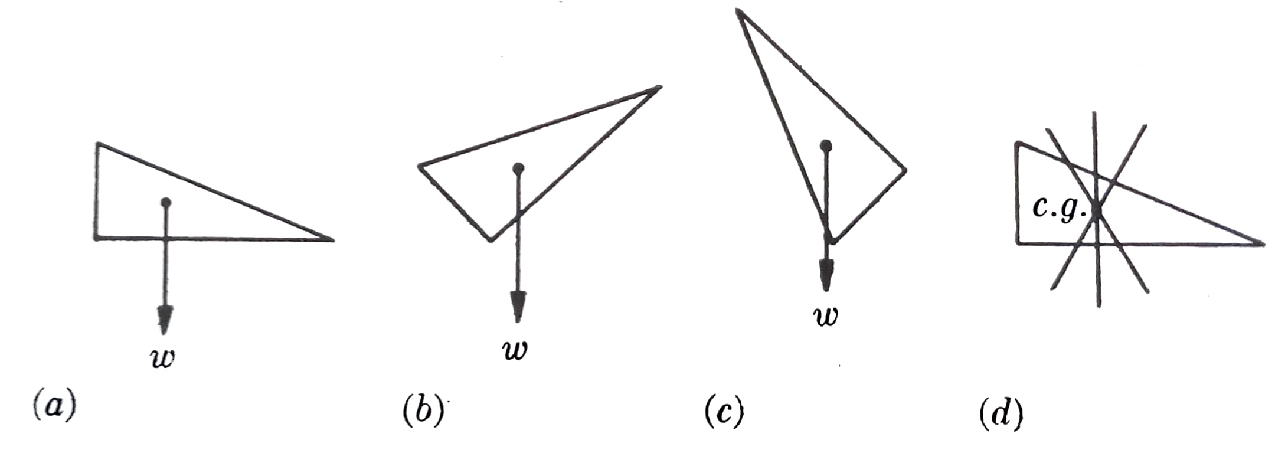
\includegraphics[width=0.8\textwidth]{/home/shluna/UNAHUR/Física/Clases/figs/centro de gravedad.pdf}
%     \end{figure}

    
% \end{frame}

% \begin{frame}{Centro de gravedad}

%     En consecuencia, el peso de un cuerpo puede considerarse como una sola fuerza cuyo punto de aplicación es el centro de gravedad. \pause

%     \vspace{11pt}

%     En realidad, el \emph{punto de aplicación} de una fuerza carece de importancia. Lo que sí se puede decir, en términos más generales, es que la línea de acción del peso (pensado como resultante) pasa siempre por el centro de gravedad.

%     \vspace{11pt}

%     \begin{block}{Propiedad importante}
%         El centro de gravedad de un cuerpo regular coincide con su centro geométrico.
%     \end{block}

        
% \end{frame}

% \begin{frame}{Centro de gravedad}

%     \begin{block}{Cálculo de la posición del centro de gravedad}
%         Para calcular la posición del centro de gravedad de un conjunto de cuerpos, se debe tener en cuenta que este es el punto de intersección de las rectas de acción de los pesos de los cuerpos que resultan de diferentes orientaciones del conjunto.
%     \end{block} \pause

%     En el plano: $$\bar{x} = \frac{\sum P_i \, x_i}{\sum P_i} \quad \text{ e } \quad \bar{y} = \frac{\sum P_i \, y_i}{\sum P_i}$$

% \end{frame}

% \begin{frame}{Pares}

%     Un caso particular e importante de fuerzas paralelas lo constituye aquél en el que se tienen dos fuerzas de igual intensidad y dirección, pero de sentido opuesto. Tal conjunto se denomina \emph{par}. \pause

%     \begin{figure}[h]
%         \centering
%         \begin{tikzpicture}[scale=1]
%             \draw[thick,latex-latex] (0,0) -- node[fill=white]{$a$} (4,0);
%             \draw[thick,latex-latex] (4,0) -- node[fill=white]{$b$} (6,0);
%             \fill[black] (0,0) circle (0.5mm);
%             \node[anchor=east] at (0,0) {$O$};
%             \draw[thick,-latex] (4,-1) -- (4,1) node[anchor=south]{$\vec{F}_1$};
%             \draw[thick,latex-] (6,-1) -- (6,1) node[anchor=south]{$\vec{F}_2$};
%         \end{tikzpicture}
%     \end{figure}

    
% \end{frame}

% \begin{frame}{Pares}

%     \begin{figure}[h]
%         \centering
%         \begin{tikzpicture}[scale=1]
%             \draw[thick,latex-latex] (0,0) -- node[fill=white]{$a$} (4,0);
%             \draw[thick,latex-latex] (4,0) -- node[fill=white]{$b$} (6,0);
%             \fill[black] (0,0) circle (0.5mm);
%             \node[anchor=east] at (0,0) {$O$};
%             \draw[thick,-latex] (4,-1) -- (4,1) node[anchor=south]{$\vec{F}_1$};
%             \draw[thick,latex-] (6,-1) -- (6,1) node[anchor=south]{$\vec{F}_2$};
%         \end{tikzpicture}
%     \end{figure}

%     $$ R = F_1 - F_2 = 0$$ \pause Es imposible producir con una sola fuerza el mismo efecto que con un par, e inversamente, no hay ninguna fuerza que pueda ser sustituida por un par.

% \end{frame}

% \begin{frame}{Pares}

%     \begin{figure}[h]
%         \centering
%         \begin{tikzpicture}[scale=1]
%             \draw[thick,latex-latex] (0,0) -- node[fill=white]{$a$} (4,0);
%             \draw[thick,latex-latex] (4,0) -- node[fill=white]{$b$} (6,0);
%             \fill[black] (0,0) circle (0.5mm);
%             \node[anchor=east] at (0,0) {$O$};
%             \draw[thick,-latex] (4,-1) -- (4,1) node[anchor=south]{$\vec{F}_1$};
%             \draw[thick,latex-] (6,-1) -- (6,1) node[anchor=south]{$\vec{F}_2$};
%         \end{tikzpicture}
%     \end{figure}

%     El único efecto de un par es producir una rotación. \pause
%     \begin{equation*}
%         \begin{split}
%             \sum T^{O} &= F_1 \, a - F_2 \left(a+b\right) \\
%                           &= F_1 \, a - F_2 \, a - F_2 \, b \\
%                           &= \left(F_1 - F_2\right) a - F_2 \, b
%         \end{split}
%     \end{equation*}

% \end{frame}

% \begin{frame}{Pares}

%     \begin{figure}[h]
%         \centering
%         \begin{tikzpicture}[scale=1]
%             \draw[thick,latex-latex] (0,0) -- node[fill=white]{$a$} (4,0);
%             \draw[thick,latex-latex] (4,0) -- node[fill=white]{$b$} (6,0);
%             \fill[black] (0,0) circle (0.5mm);
%             \node[anchor=east] at (0,0) {$O$};
%             \draw[thick,-latex] (4,-1) -- (4,1) node[anchor=south]{$\vec{F}_1$};
%             \draw[thick,latex-] (6,-1) -- (6,1) node[anchor=south]{$\vec{F}_2$};
%         \end{tikzpicture}
%     \end{figure} En consecuencia, $$\sum T^{O} = - F_2 \, b = - F_1 \, b$$ Es decir, el momento de un par es siempre igual al producto del módulo de \emph{cualquiera} de las fuerzas por la distancia entre las rectas de acción.

% \end{frame}

% \section{Rotación y traslación} 

% \begin{frame}{Rotación y traslación}



% \end{frame}

\begin{frame}{Esto es todo por hoy}

    \begin{center}
        {\huge ¡Muchas gracias!}

        \vs

        Ahora a repasar y practicar.
    \end{center}

\end{frame}

\end{document}

\begin{frame}{}



\end{frame}